\documentclass{exam}
\author{Nima Poshtiban}
\title{Digital Electronics}
\usepackage{datetime}
\newdate{date}{26}{10}{2025}
\newdate{due}{1}{11}{2025}
\date{\displaydate{date}}
\usepackage[utf8]{inputenc}
\usepackage{amsmath}
\usepackage{enumitem}
\usepackage{graphicx}
\usepackage[urlcolor=blue, bookmarksopen]{hyperref}
\usepackage[]{geometry}
\usepackage[]{cleveref}
\usepackage{amsmath}
\usepackage{xcolor}
\usepackage{siunitx}
\usepackage{tikz}
\usepackage{svg}

\begin{document}
\maketitle
\tableofcontents 
\pagebreak

\section{Assignment No.1}
\begin{center}
\fbox{\fbox{\parbox{5.5in}{\centering
Assignment Due: \displaydate{due}}}}
\end{center}


\begin{questions}
\question Draw the schematics of an Exclusive OR (XOR) using \textbf{MOSFETs} (\textbf{BJTs are prohibited})

\paragraph{}
\begin{figure}[httb]
 	\centering
\includegraphics[scale=0.5]{xor.pdf}

\end{figure}

\question Run the given HDL file and report back the results (Screenshots are Mandatory)
\paragraph{}
\textbf{Thanks to hyper-V }
\begin{figure}[h]

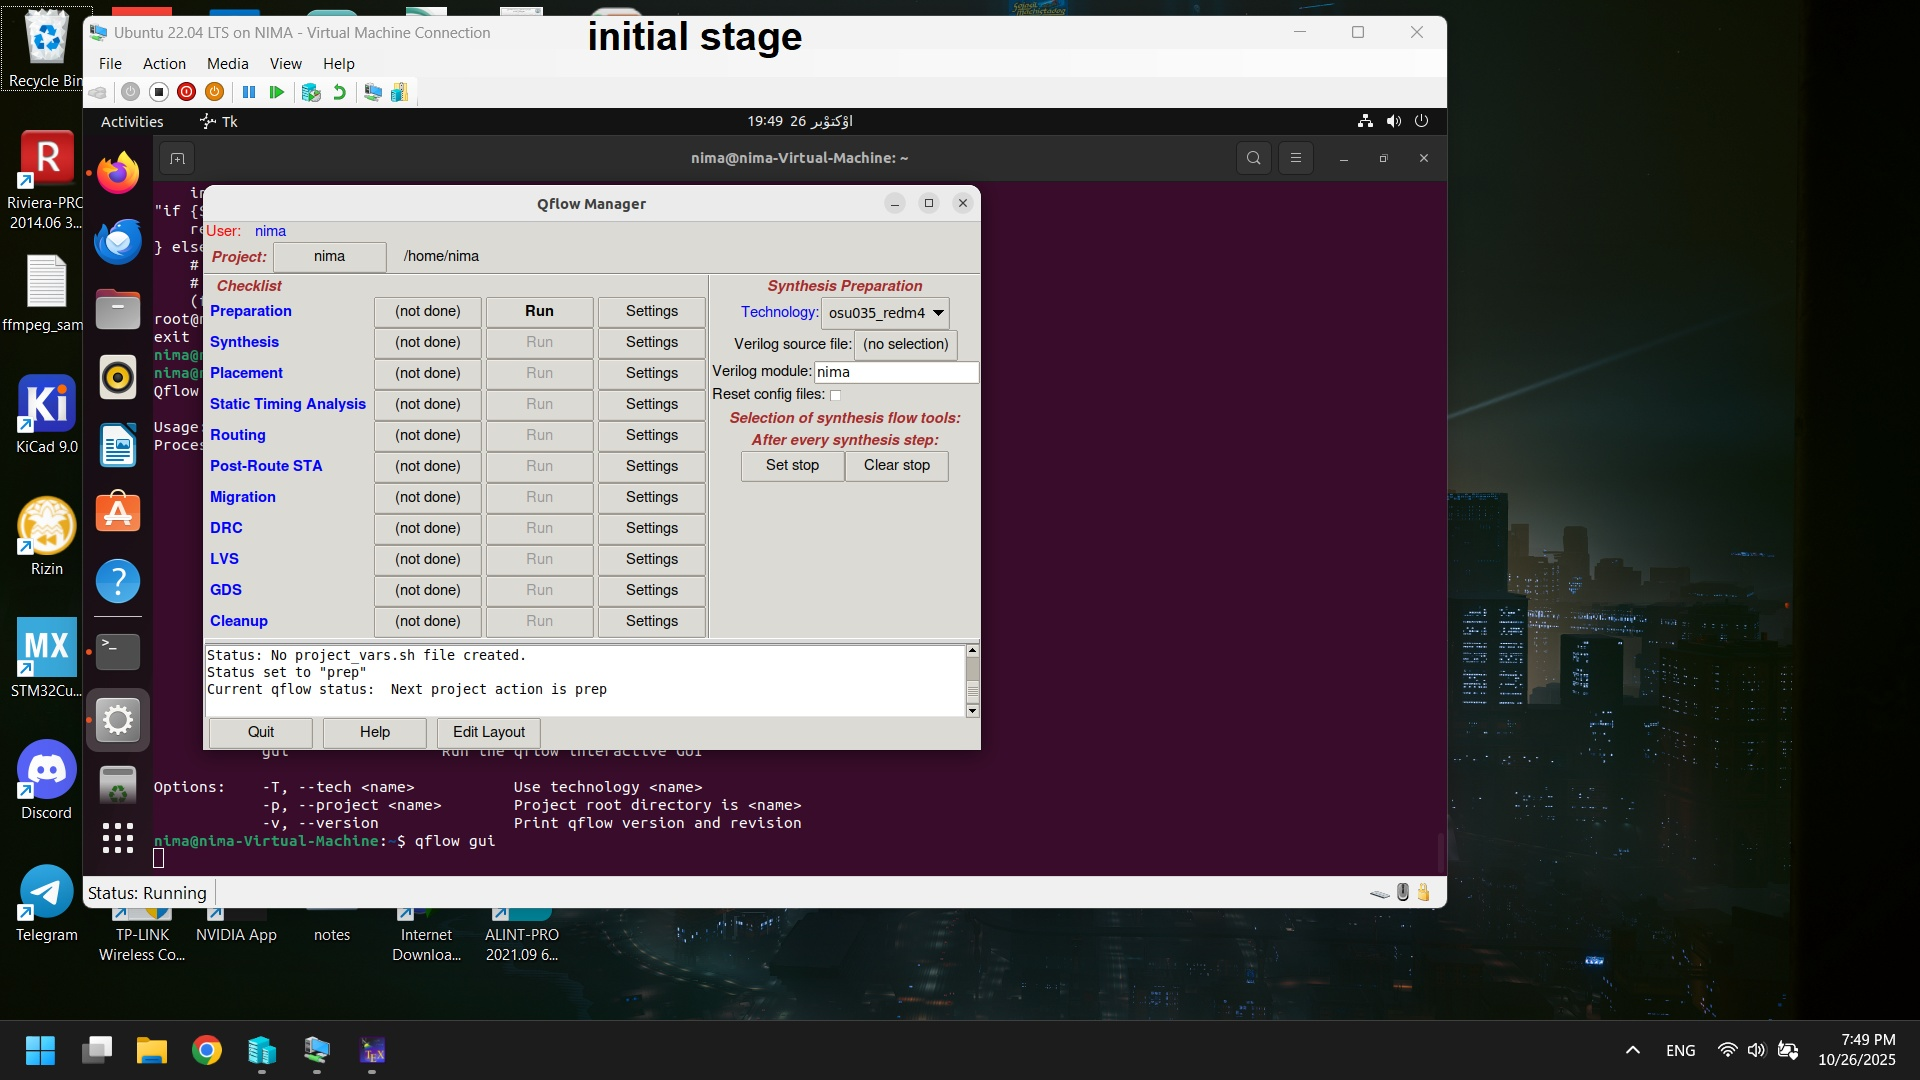
\includegraphics[scale=0.2]{init.jpg}
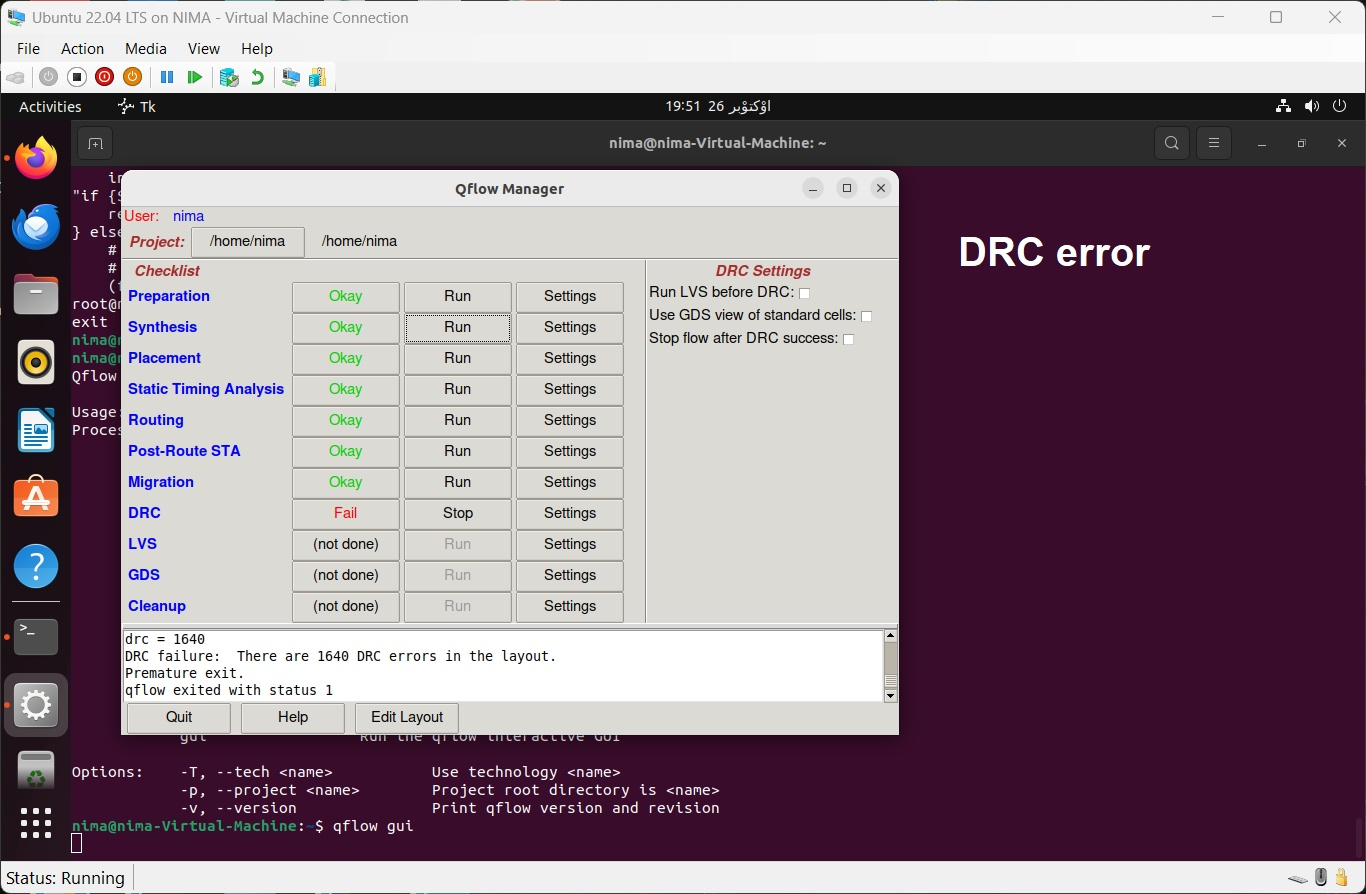
\includegraphics[scale=0.2]{drc.jpg}
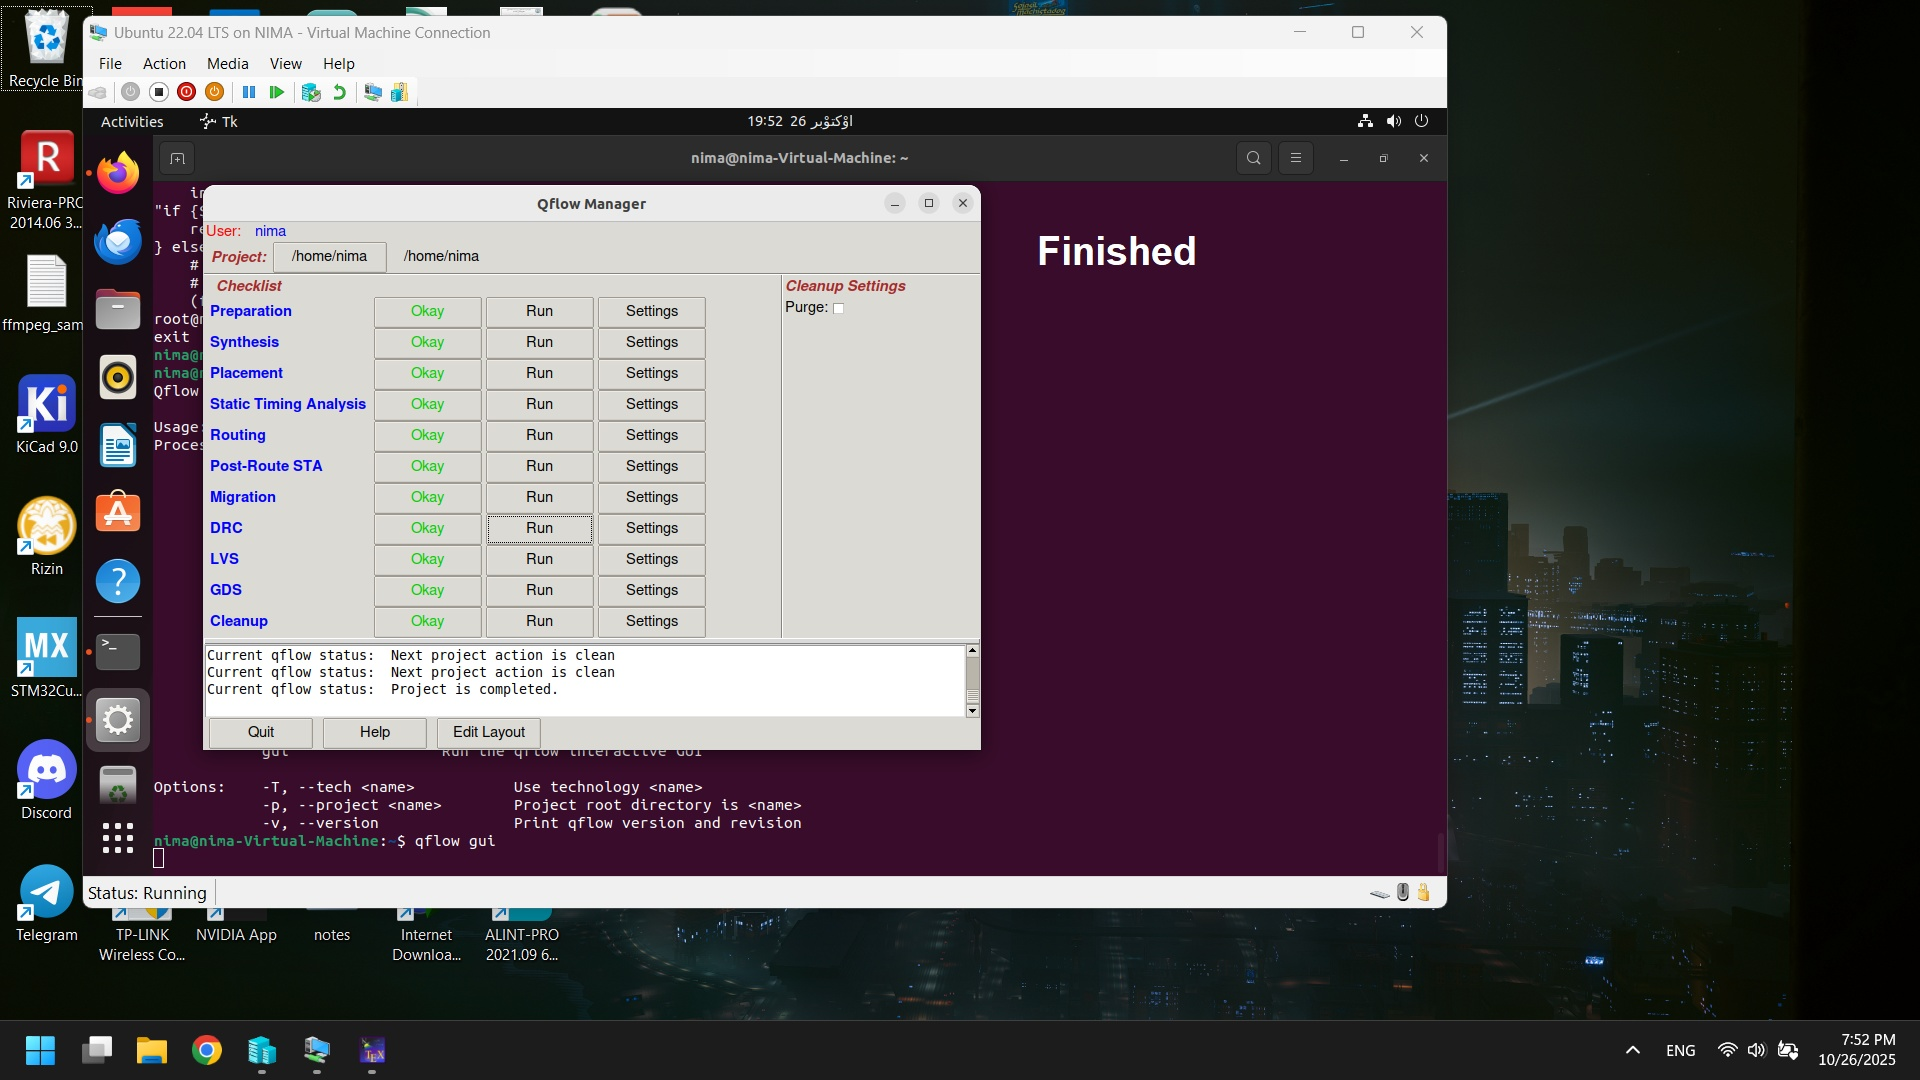
\includegraphics[scale=0.2]{finished.jpeg}
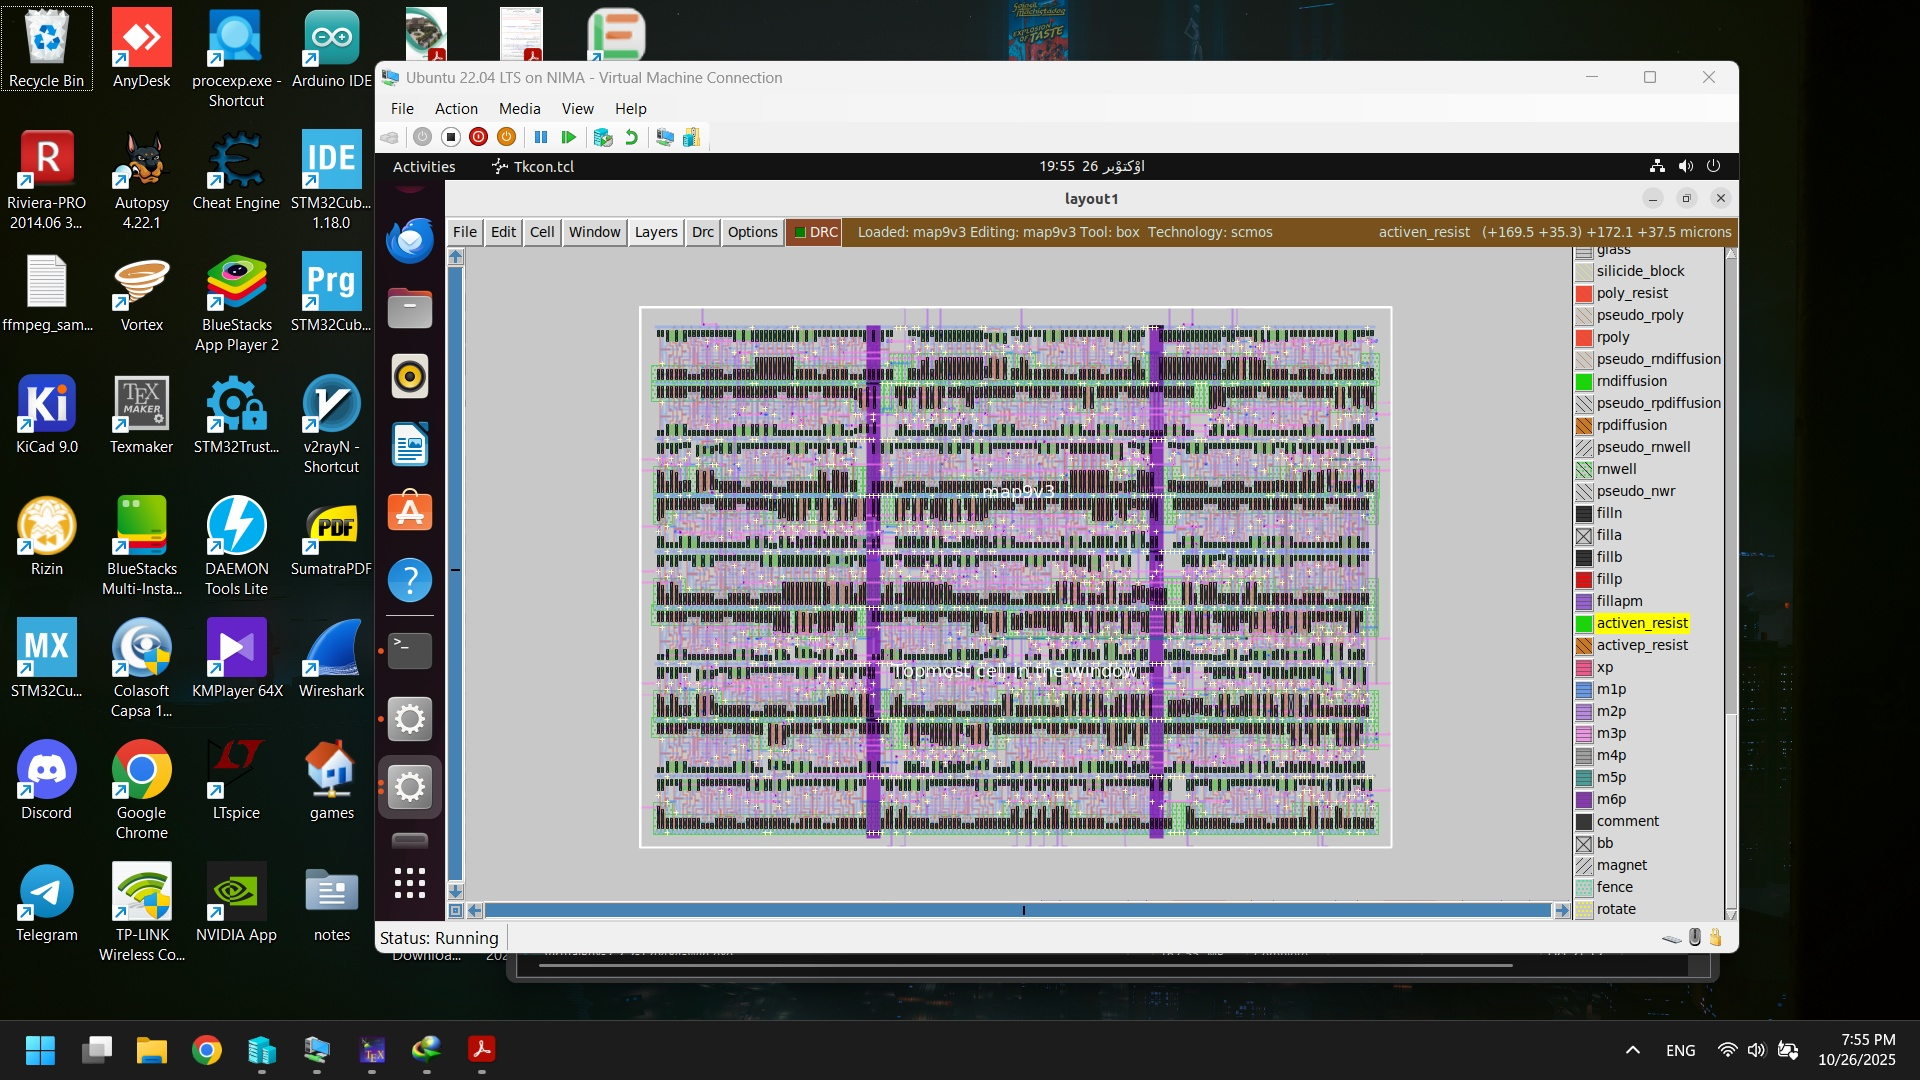
\includegraphics[scale=0.2]{layout.jpg}
\end{figure}

%todo add and complete ordinary questions


\end{questions}


\end{document}